\ifdefined\included
\else
\setcounter{chapter}{8} %% Numéro du chapitre précédent ;)
\dominitoc
\faketableofcontents
\fi

\chapter{A robot in the mall: The MuMMER project}
\minitoc

This chapter is a sum-up of an article submitted to the  User Modeling and User-Adapted Interaction (UMUAI) Journal. This work has been achieved in collaboration with Amandine Mayima, Guilhem Buisan, Phani-Teja Singamaneni, Yoan Sallami, Kathleen Belhassein, and Jules Waldhart. In this chapter, we first give an overview of the European H2020 Project \acrfull{mummer}\footnote{\url{http://mummer-project.eu/}}, in the context of which the contribution of chapter~\ref{chap:3} was made. We then present the components developed by the LAAS-RIS team with a focus on the component in which I participated as well as their integration in a robotic architecture.

\section{Introduction}

In large scale, indoor environments, like museums, shopping malls, or airports, the presence of large interactive screens, maps, or signs underline the importance of providing information on itineraries. However, reading such maps can be challenging and some information can be missing like the location of the shops selling a given product. To bring such new information and help people to find their itinerary in large indoor environments such as shopping malls, robots can be used.

To study this challenge and the underlined Human-Robot Interaction requirement, in the context of the European H2020 Project \acrshort{mummer}~\cite{foster_2016_mummer}, we have developed and deployed a social service robot in one of the largest malls of Finland, Ideapark in the city of Lemp\"a\"al\"a. The resulting robot is able to chat with customers and guide them. The chatting has been brought by a partner of the project. The contribution of the LAAS-RIS team, and thus the focus of this chapter, was on the direction-giving task.

With a mall having approximately 1.2 kilometers of pedestrian streets and more than 150 shops, having a robot accompanying customers would be time-consuming. Taking inspiration from the mall employees, we chose to verbally describe the route while grounding it with pointing gestures. The robot can however move a few meters if needed. %Such a movement can be useful to improve the perspective sharing of landmark to better ground the route description.
The output of this project is a complete robot architecture that integrates a number of components. Each of them makes use of various models and decisional algorithms, all integrating explicitly human models.

First, we provide background information about robot guides and discuss how the human partner has been considered. Then, we present the human-human exploratory studies used to identify the required abilities for a guide robot. We then present the developed architecture and its components. We end this chapter with integration on a real robotic system with some detail on its deployment "into the wild".

\section{Related work}

A number of contributions have proposed robot guides, from the first museum guides \cite{burgard_1999_museum, siegwart_2003_robox, clodic_2006_rackham} to more recent robot guides in large areas \cite{bauer_2009_autonomous, triebel_2016_spencer}. A recent example is presented in \cite{chen_2017_robots}. The developed robot is able to accompany the customer to its destination, then to point at it. Another robot presented in \cite{gross_2009_toomas} can help the customer to find specific product among all the shops of a mall. Most of these works are focused on the navigation aspect of the task. It requires environment mapping, localisation, and social navigation due to the presence of many humans.

Where previous contributions were mostly focused on navigation, others have investigated the direction-giving task, meaning the fact to not accompany the customer but to describe the route to the goal. For example, \cite{cassell_2007_trading} describes an embodied conversational agent giving route directions using deictic gestures. Within the Robovie project, the ATR-IRC laboratories have developed a robot providing route description through the use of utterances and gestures, and have highlighted the importance of their timing~\cite{okuno_2009_providing}. Kanda et al. in \cite{kanda_2009_affective} and \cite{kanda_2010_communication} have divided the direction giving into two steps. First the robot point toward the direction to take, then it explains the full route. In addition, the robot can give recommendations for restaurants and shops. Finally, \cite{satake_2015_should} showed a complete architecture of an information-providing robot able to move around a square in a mall. It embedded a map, an ontology, a speech recognition system, a dialog manager, a localization module, and a people tracker. As in their previous works, the robot verbalized utterances and used deictic gestures to give route directions. Numerous other contributions can be found but, only a few of them propose full architectures for an autonomous direction-providing robot, the most complete one being the Robovie robot presented above. 

To the best of our knowledge, no system tackles the guiding-task by reasoning about the shared perspective. If the robot has to point a landmark not visible by the human at its current position, we want the robot to pro-actively propose to the human a pertinent placement. This is one of the basic bricks of our system and it is strongly linked to the key principles of Joint Action which involve the ability to establish and monitor joint attention~\cite{pacherie_2012_phenomenology}.

\section{Learning from exploratory studies}

To lead to robot abilities design and implementation, two human-human exploratory studies were conducted in collaboration with VTT Technical Research Centre of Finland. In addition to the current literature, it allows us to enrich our knowledge with effective route descriptions in the robot deployment environment.

The first pilot study consisted of a human guide providing route information. It consisted of one participant asking for shop directions to a guide working at the mall information booth. The analysis focused on gestures used to give guidance, the positions of the two protagonists in relation to the target shop and their interlocutor, and the gazes alternation. \cite{belhassein_2017_human} gave the first indications to consider resulting from this pilot study. Among these results, we can note a preference over the ipsilateral hand to the visual field of the target. This study also provides numbers of dialogue transcription use to study how guides effectively provide route description and give examples of descriptions.

\begin{figure}[ht!]
\centering
\includegraphics[scale=0.35]{figures/chapter8/human_guide.png}
\caption{\label{fig:chap8_human_guide} Picture from the second Human-Human study \cite{belhassein_2017_human}. Here, the guide is giving the route description to reach a given shop by pointing at it. The formation formed by the guide, teh customer, and the target were analyzed. }
\end{figure}

A second exploratory study was then carried out to focus on more complex situations. Among them, we can note situations with two customers requesting directions simultaneously, a customer requesting for two shops at the time, or someone interrupting an ongoing interaction. Once again the formations were analyzed. An example of such a formation seen during the study can be seen in figure~\ref{fig:chap8_human_guide}. The full results can be found in~\cite{Heikkilae_2018_where} and~\cite{heikkilae_2019_should}. Among these results, the study has shown that the guide usually points to the general location of the target first and in a second step explain and point the different stages of the route.

\section{The deliberative architecture}

\begin{figure}[ht!]
\centering
\includegraphics[width=\textwidth]{figures/chapter8/architecture.png}
\caption{\label{fig:chap8_architecture} todo. }
\end{figure}

\subsection{Environment representation}

\subsubsection{Geometric representation}

\begin{figure}[ht!]
\centering
\includegraphics[scale=0.15]{figures/chapter8/adream_base_m.png}
\caption{\label{fig:chap8_adream_base} todo. }
\end{figure}

\begin{figure}[ht!]
\centering
\includegraphics[scale=0.15]{figures/chapter8/ideapark_base_m.png}
\caption{\label{fig:chap8_ideapark_base} todo. }
\end{figure}

\subsubsection{Semantic representation}

\begin{figure}[ht!]
\centering
\includegraphics[scale=0.45]{figures/chapter8/zizzi.png}
\caption{\label{fig:chap8_zizzi} todo. }
\end{figure}

\subsection{Perceiving the partner}

\subsection{Generating route description}

\subsection{Planning a shared visual perspective}

\begin{figure}[ht!]
\centering
\includegraphics[scale=0.25]{figures/chapter8/grid_map.png}
\caption{\label{fig:chap8_svp_grid} todo. }
\end{figure}

\begin{figure}[ht!]
\centering
\includegraphics[scale=0.45]{figures/chapter8/svp.png}
\caption{\label{fig:chap8_svp} todo. }
\end{figure}

\subsection{Navigate close to the human}

\subsection{Executing and controling the task}

\section{Embody architecture in a physical robot}

\subsection{Pepper in Ideapark}

\begin{figure}[ht!]
\centering
\includegraphics[scale=0.15]{figures/chapter8/pepper_mall.png}
\caption{\label{fig:chap8_pepper_mall} todo. }
\end{figure}

\subsection{Pepper "in the wild"}